%TC:ignore

\chapter{CRC Cards}
\label{appendix:crc-cards}

The following \acrshort{CRC} Cards are only an outline of the most important functions and scripts in the project. Other, less-important, existing functions/scripts may be referred to in the collaboration section.

\begin{figure}[H]
  \center
  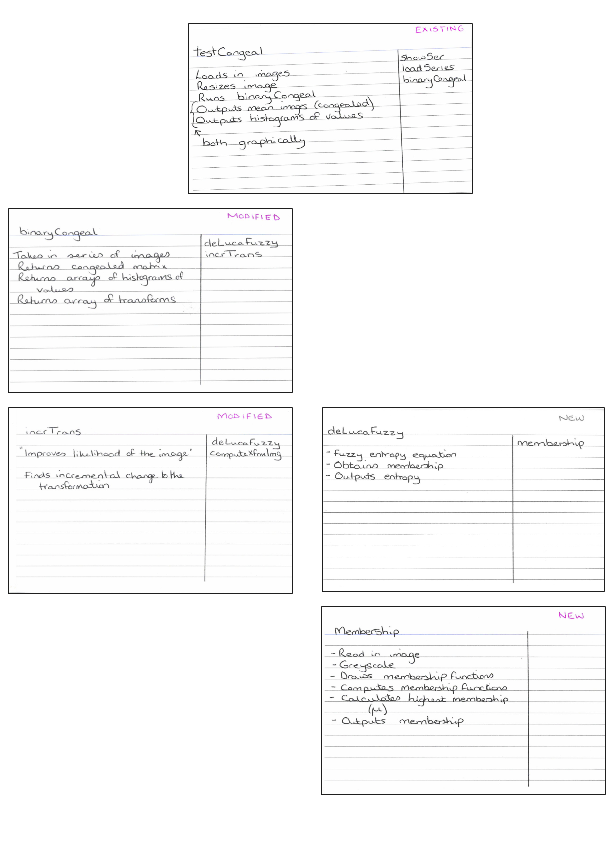
\includegraphics[scale=0.5]{Appendix4/imgs/initial.png}
  \caption{Initial design}
  \label{fig:initial-design}
\end{figure}

Figure \ref{fig:initial-design} details the initial planned design for the implementation of De Luca \& Termini's Non-Probabilistic entropy. The top-down structure represents the order in which the scripts or functions were called, with testCongeal being the function run by the user.

\begin{figure}[H]
  \center
  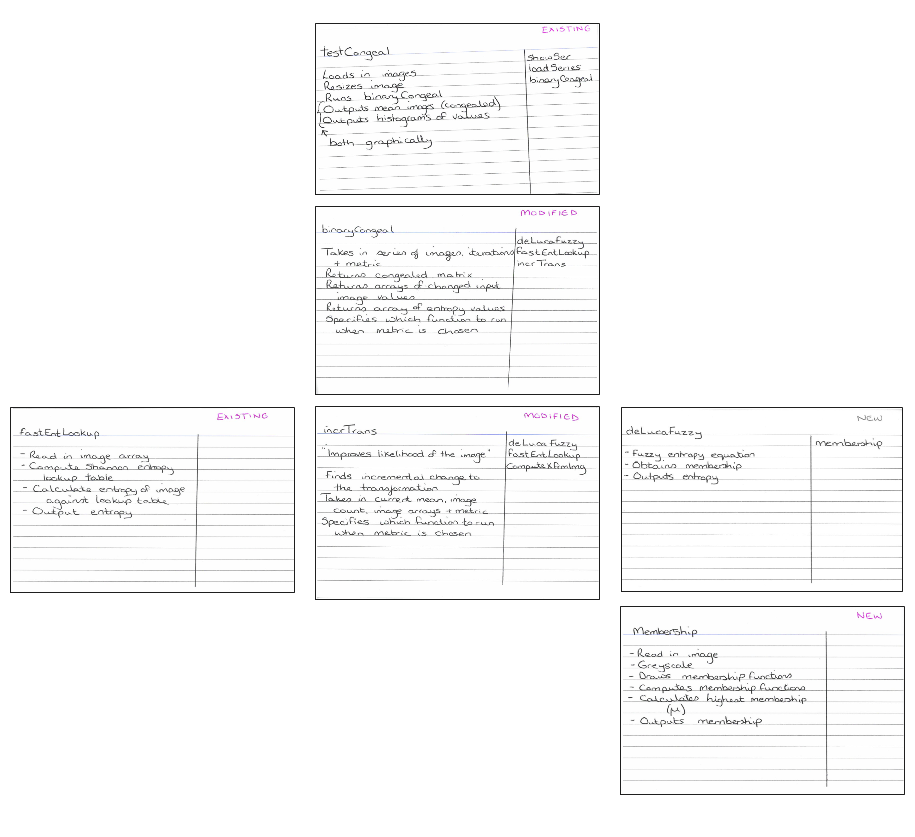
\includegraphics[scale=0.5]{Appendix4/imgs/second.png}
  \caption{Secondary design}
  \label{fig:second-design}
\end{figure}

Figure \ref{fig:second-design} shows the second design iteration. Note the change in \texttt{incrTrans} and \texttt{binaryCongeal} CRC cards, and the addition of \texttt{fastEntLookup} when Learned-Miller`s Shannon Entropy metric is reintroduced.

\begin{figure}[H]
  \center
  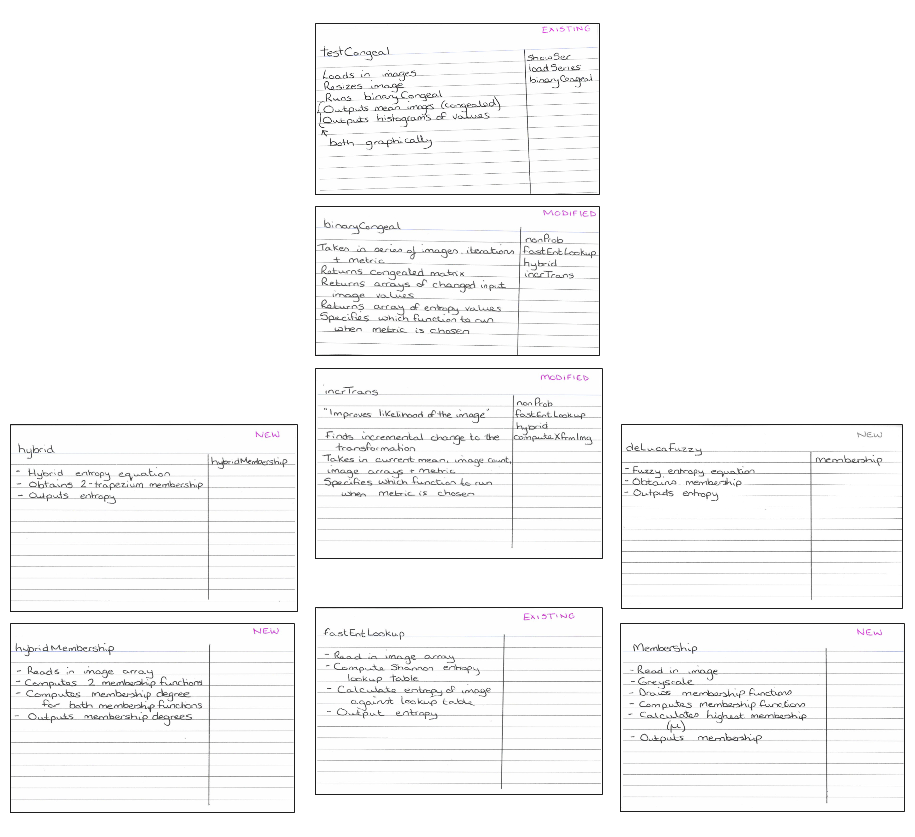
\includegraphics[scale=0.5]{Appendix4/imgs/third.png}
  \caption{Third design}
  \label{fig:third-design}
\end{figure}

Figure \ref{fig:third-design} represents the third iteration. The new \texttt{hybrid} and \texttt{hybridMembership} functions have been added, and \texttt{binaryCongeal} and \texttt{incrTrans} have once again been updated to reflect this.

\begin{figure}[H]
  \center
  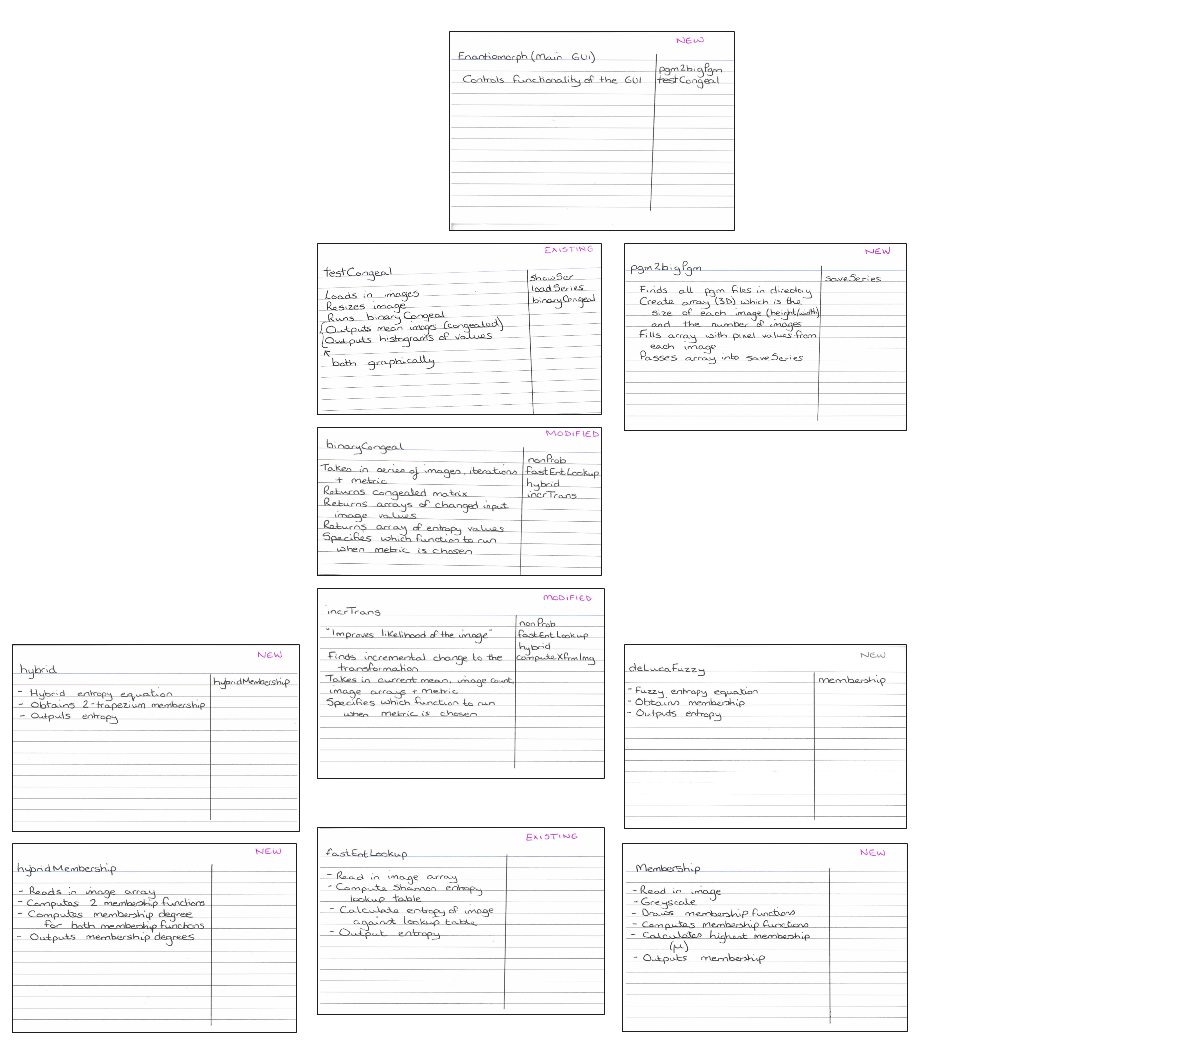
\includegraphics[scale=0.5]{Appendix4/imgs/fourth.png}
  \caption{Fourth design}
  \label{fig:fourth-design}
\end{figure}

Figure \ref{fig:fourth-design} shows the addition of the \acrshort{GUI} element, called \texttt{Enantiomorph} and also the function designed to handle the concatenation of mammogram pgm files \texttt{pgm2bigPgm}.

\begin{figure}[H]
  \center
  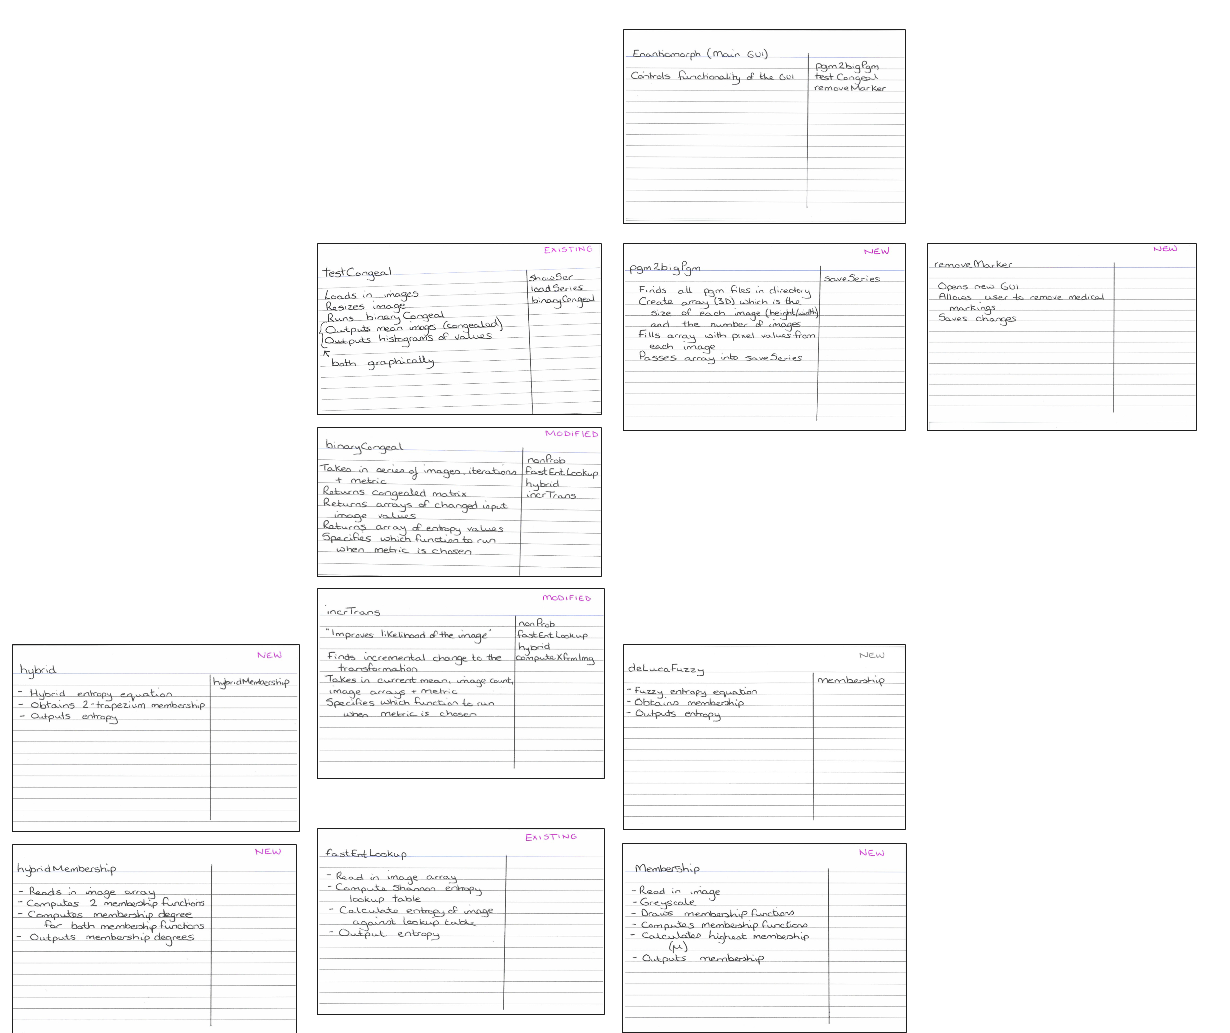
\includegraphics[width = \textwidth]{Appendix4/imgs/final.png}
  \caption{Final design}
  \label{fig:final-design}
\end{figure}

Figure \ref{fig:final-design} is the final high-level design of the system. It includes the addition of the secondary \acrshort{GUI}, \texttt{removeMarker} which handles the removal of any medical markings from the mammograms.

%TC:endignore
